\documentclass[main.tex]{subfiles}
\begin{document}
\section{Analysis}
From the output of a single block encrypted with DES, we can see that it does
not have sufficient confusion for the last bit. Changing the last bit of the key
has no effect on the cipher text. However, the cipher has strong properties of
diffusion, as changing even a single bit of the plaintext significantly changes
the ciphertext.

It is also observed that the subsitution part of the encryption algorithm
ensures that an all-zero key and message do not lead to an all-zero ciphertext
showing that the algorithm is not linear in its inputs.

\lstinputlisting[style=codeStylePy3]{des.py}
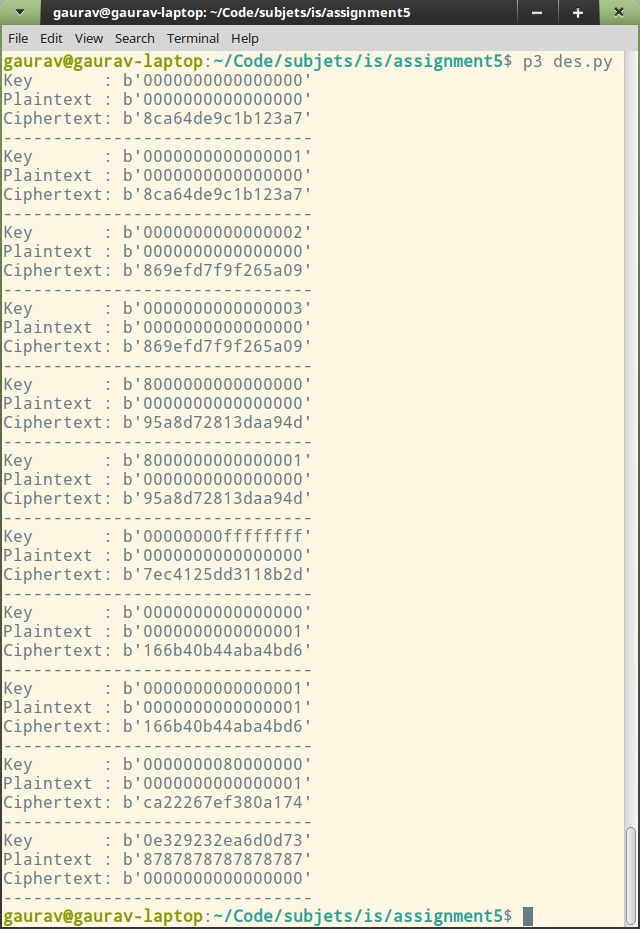
\includegraphics[width=\textwidth]{output.png}



\end{document}
